\chapter{Background}
% Maybe split into two chapters?

\label{chap:refs}

\section{Machine learning fundamentals}

Our goal is to optimize hyperparameters, but before we introduce the main topic, we need to specify the context --- machine learning. Even though we suspect that most readers are already familiar with machine learning, we include it for completeness and to introduce the notation. We encourage readers familiar with machine learning, and with deep learning in particular, to skip this section. First, we will introduce the task of supervised machine learning, how the dataset is commonly split, and the function that is optimized in order to train the model. Then we will briefly introduce deep learning and a couple of frequently used architectures. Finally, we will end with an overview of the optimization algorithm behind neural networks. We hope to give the reader some intuition behind the optimization problem of hyperparameter search without going into unnecessary detail.

% In general, machine learning is the ability of an AI system to acquire its own knowledge by extracting patterns from raw data. In the last decade, one particular class of machine learning algorithms took over --- deep learning.

%Before we get to hyperparameters and optimization, we will revisit and define key concepts from machine learning so that it is clear what machine learning models we use and why.


% Briefly revisit deep neural networks and ML

% Machine learning applications - should I introduce machine learning in general? I think everyone has to know

\subsection{Supervised machine learning}
% Dataset, labeled examples, classification vs regression
Let $\mathcal{D}$ be a labeled dataset, consisting of examples generated independently from a data-generating distribution. Each example $(x^{(i)}, \  y^{(i)})$ consist of a feature vector $x^{(i)}\in \mathcal{X}$ and its label $y^{(i)}\in \mathcal{Y}$. Depending on the labels, we distinguish classification and regression. In classification, the labels are finite-valued, while in regression the labels are real numbers. The goal of supervised learning is to train a model using the examples from the dataset $\mathcal{D}$ so that it generalizes well to data from the data-generating distribution. Simply put, we want the model to correctly predict the labels on unseen data. We assume the unseen data come from the same data-generating distribution so that the model can use the learned patterns for the task.  % Generalization error

% Generalization, train, val, test split
Since the goal is for the model to generalize well, we need to estimate the generalization error in the training and model selection process on unseen data. It is a best practice to split the dataset into $\mathcal{D}_{train}, \  \mathcal{D}_{val}, \mathcal{D}_{test}$. We use $\mathcal{D}_{train}$ for the training of the model, $\mathcal{D}_{val}$ for the estimate of the generalization error during development, and $\mathcal{D}_{test}$ for the final evaluation. A separate test set is needed for the final evaluation because the validation set has already been used to choose the best model, which means there is a bias in the estimate. As we will see, using a hyperparameter optimization tool introduces yet another optimization layer, meaning we should do a similar split even for the outer optimization of hyperparameters.


% Training - minimizing the loss function
We train machine learning algorithms by minimizing the loss function on the training data. Two loss functions are used most commonly. For regression, the mean square error of $N$ examples is computed as $$ MSE=\frac{1}{N} \sum_{i=1}^{N} (f(x^{(i)});\theta )-y^{(i)})^2.$$

% Cross entropy loss, MSE loss
In the case of classification, we use the cross-entropy loss that measures the difference between two probability distributions. Let $C$ be the number of classification classes and let $y^{(i)}$ be a distribution over all classes, which will often be just a one-hot encoding of the target class. Let the predictions of the model also form a distribution over the classes. Then the loss is calculated as follows when using mean reduction across examples $$CE=-\frac{1}{N} \sum_{i=1}^{N} \sum_{c=1}^{C} y^{(i)}_c log(f(x^{(i)});\theta )_c\, .$$

% More about the loss, metrics
The loss functions depend mostly on the task, not on the specific machine learning model. The training algorithm that optimizes the loss function depends on the model though, so we will revisit optimization later. Even though the training is done exclusively with the loss function, we do not need to use the loss function for the evaluation of the model. Oftentimes a better metric, such as classification accuracy, is used instead. That holds even for hyperparameter optimization; we can optimize hyperparameters for any metric.

% We focus on hyperparameter optimization of neural networks since neural networks are widely used today and have many hyperparameters.
\subsection{Deep learning}
% Deep learning, perceptrons
Deep learning is the subset of machine learning methods based on neural networks. The ``deep'' in deep learning refers to the use of multiple layers in the network. A neural network describes a computation. The basic unit is called a node and the nodes are arranged in an acyclic graph. Nodes generally represent some operation, while edges can be annotated with parameters for the operation. We call the parameters or neural network weights. A simple example of a neural network is the perceptron (see Figure~\ref{fig:perceptron}). The output value is computed by summing the values of inputs multiplied by the corresponding weights, adding a bias of the node, and passing the weighted sum through an activation function $a$:
$$ y = a(\sum_j x_jw_j + b).$$

\begin{figure}
\centering
\begin{tikzpicture}[
    neuron/.style={circle, draw, minimum size=9mm, inner sep=0pt},
    input/.style={circle, draw, minimum size=9mm, fill=blue!30, inner sep=0pt},
    output/.style={diamond, aspect=2, draw, minimum size=9mm, fill=green!30, inner sep=0pt},
    sum/.style={circle, draw, minimum size=9mm, fill=purple!30, inner sep=0pt},
    activation/.style={circle, draw, minimum size=9mm, fill=red!30, inner sep=0pt},
    >=stealth
]

% Inputs
\node[input] (x1) {$x_1$};
\node[input, below=0.4cm of x1] (x2) {$x_2$};
\node[input, below=0.4cm of x2] (x3) {$x_3$};
\node[input, below=0.4cm of x3] (x4) {$x_4$};

% Weighted sum node
\node[sum, right=of x2, xshift=1.5cm, yshift=-0.4cm] (sum) {$\sum$};

% Activation function node
\node[activation, right=1.5cm of sum] (activation) {};

% Output node
\node[output, right=1.5cm of activation] (output) {$y$};

% Connections
\draw[->] (x1) -- node[midway, above, xshift=-0.1cm] {$w_1$} (sum);
\draw[->] (x2) -- node[midway, above, xshift=-0.1cm] {$w_2$} (sum);
\draw[->] (x3) -- node[midway, above, xshift=-0.1cm] {$w_3$} (sum);
\draw[->] (x4) -- node[midway, above, xshift=-0.1cm] {$w_4$} (sum);
\draw[->] (sum) -- (activation);
\draw[->] (activation) -- (output);

% Labels
\node[above=0.2cm of x1] {Inputs};
\node[above=0.5cm of sum] {Weighted Sum};
\node[above=0.2cm of activation] {Activation Function};
\node[above=0.5cm of output] {Output};

\end{tikzpicture}

\caption{Perceptron neural network}
\label{fig:perceptron}

\end{figure}

% MLP

% Multi-layer perceptron
We can reuse this basic building block (weighted sum with bias followed by an activation function) and combine it to form a larger network. If we stack several such blocks, or nodes,  on top of each other, we get a \textit{fully connected layer}. It gets its name from the fact that each node in the layer is connected to every input node. If we connect another fully connected layer to the outputs of the first, we get an architecture called a \textit{multilayer perceptron} (MLP). The multilayer perceptron is a good choice for tabular datasets where the features are structured as rows and columns and there are non-linear relationships between the features. The hyperparameters of MLP could be the number of hidden layers, the sizes of the individual layers, or the activation function of the hidden units.

% CNN
For image data or any other data with some structure, a \textit{convolutional neural network} (CNN) might be a good option. The basic building block of CNNs is a convolution layer. We can imagine a convolution layer as a sliding window, or a tile, that locally weights and sums the data, as illustrated in Figure~\ref{fig:conv}. The parameters of the tile, its size and the weights, are specified by the \textit{kernel}. There can be several kernels of the same size stacked on top of each other, each producing one \textit{channel} of the output. The power of CNNs comes from the fact that they learn the features gradually and combine lower-level features as each kernel processes only a small local neighborhood at a time, into higher-level features as the context window gets wider. Suppose we have two-dimensional data. Formally, the convolution layer computes the following function with kernel $K$ on input $I$ with $c$ channels to get an output value at coordinates $i,j$:
\[
 (K \ast I)_{i,j} =\sum_{m,n,c} I_{i+m,j+n,c}K_{m,n,c}\,.
\]

\begin{figure}
    \centering
    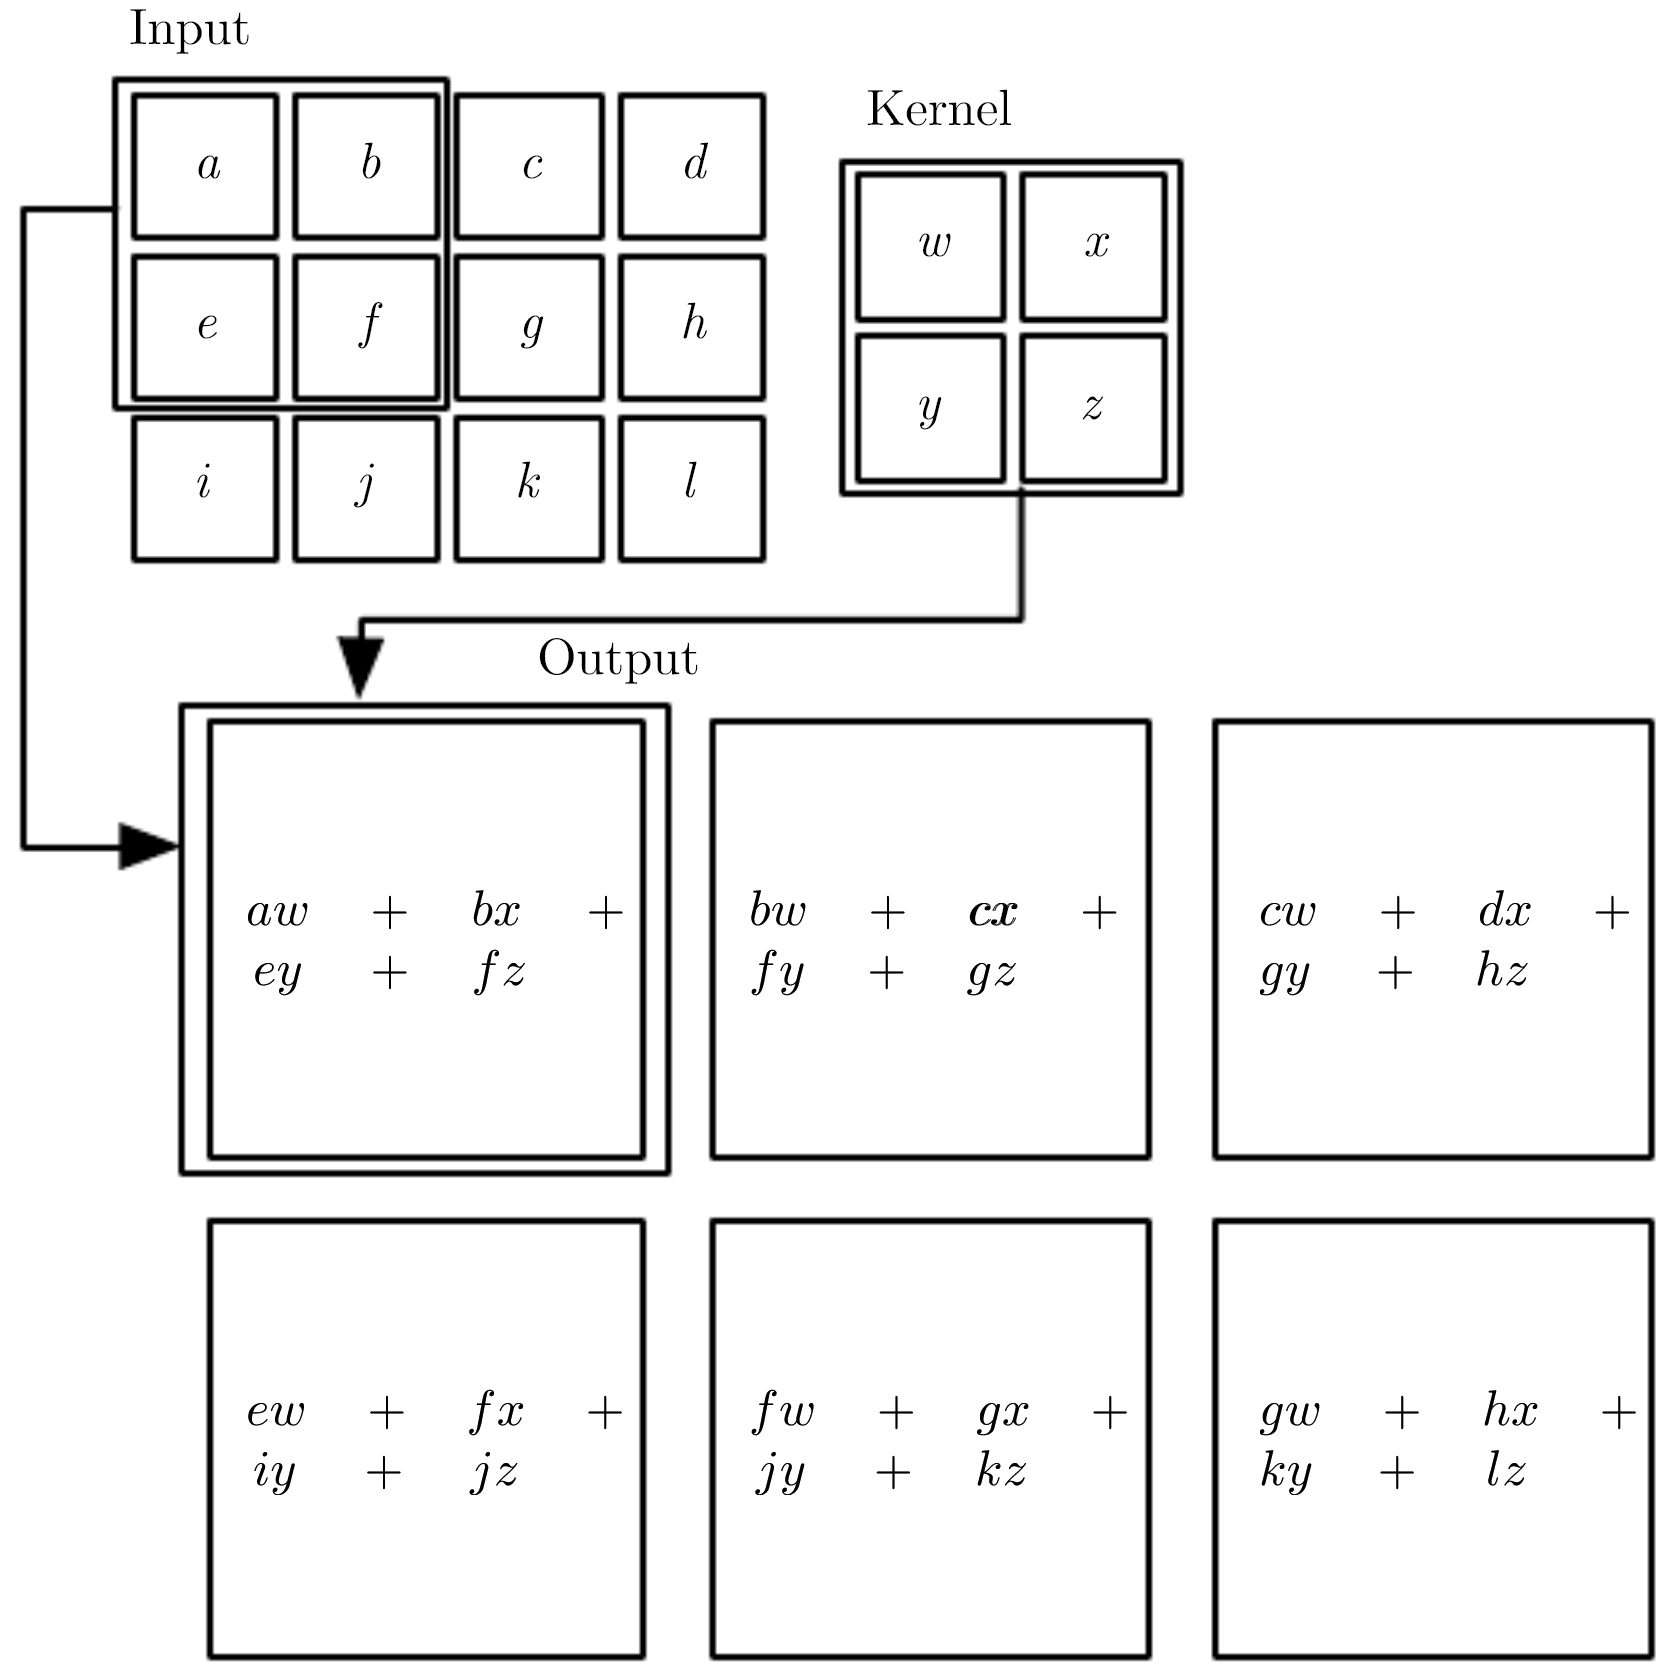
\includegraphics[scale=0.25]{img/convolution.png}
    \caption{An example of a 2-D convolution. (Source: Figure 9.1 of ``Deep Learning'' book~\cite{Goodfellow-et-al-2016})}
    \label{fig:conv}
\end{figure}

% RNN
\xxx{TODO RNNs.} The recurrent neural network is designed to handle sequential or time series data.

% Transformers

\subsection{Training of neural networks}
% Training of neural networks.
Training of the network can be split into two parts --- the forward pass and the backward pass. These two operations are repeated over and over again until some stopping criterion is met. We call one iteration an epoch. In an epoch, the training algorithm iterates through all examples in the training set, usually grouped in batches. In the forward pass, the network produces an output from the input examples and weights by iteratively going through the graph in a topological order. The loss is calculated from the output of the network and true labels. The gradients of the loss function are computed using the backpropagation algorithm, which iterates through the nodes in reverse order and calculates partial derivatives of the loss with respect to the individual weights.

% Gradient descent algorithm
After the gradients are computed, the loss function is minimized using the gradient descent algorithm. Given a loss function $L(\theta)$ that we want to minimize with respect to the weights, the gradient descent optimizes the function by taking a step in the opposite direction of gradient $\nabla_\theta L(\theta)$, which decreases the loss. That is, the weights are updated using a learning rate hyperparameter $\alpha$: $$ \theta \leftarrow \theta - \alpha \nabla_\theta L(\theta).$$

For this thesis, it is enough to know there is a gradient descent algorithm optimizing the loss and this algorithm and its more advanced derivatives, such as Adam, comes with some hyperparameters. These usually include a learning rate, a \textit{momentum}, or a \textit{decay schedule}, if we want to gradually decrease the learning rate. Later, we will also use the fact that training of neural networks is an iterative process, and it usually takes at least tens of epochs until the network starts to converge.

\subsection{Regularization}
% What is regularization
The last concept that is useful to know about for hyperparameter optimization is \textit{regularization}. It is a technique to prevent \textit{overfitting}, which is a situation when the model learns too much from the training set and the validation loss starts increasing because the model learns specific patterns present only in the training dataset. Remember we want the model to generalize well. Regularization is especially important for smaller datasets. There are many regularization techniques and most of them come with some hyperparameter. We call them regularization hyperparameters.

% Examples of regularization
One way to reduce overfitting is to use a \textit{weight decay}, which multiplies the weights by some constant smaller than one and usually close to zero, which we set as a hyperparameter. The intuition behind weight decay is that the network forgets a little each time the weights are updated, so it can learn only general patterns that occur often. Another common regularization technique is the \textit{dropout}. In dropout, some nodes are deactivated during a forward pass with the dropout rate (probability), which is a hyperparameter. The network is forced to work reasonably well with only a subset of nodes, which should also force it to learn general features.


\section{Hyperparameter optimization}
% Define hyperparameters, their impact on model performance, why optimization is important

% TODO: Definition is inspired by Towards an Empirical Foundation for Assessing... Eggensperger
Let $A$ be a machine learning algorithm with hyperparameters $\lambda_1, \dots , \lambda_n$ with domains $\Lambda_1,\dots , \Lambda_n$. Let $ \mathbf{\Lambda } = \Lambda_1 \times \cdots \times \Lambda_n$ denote its hyperparameter space. Hyperparameters can be continuous, integer-valued, or categorical. Also, we can have conditional hyperparameters. We say that hyperparameter $\lambda_i$ is \emph{conditional} on another hyperparameter $\lambda_j$, if $\lambda_i$ is only active if hyperparameter $\lambda_j$ takes values from a given set $V_i(j) \subset \Lambda_j$

For each hyperparameter configuration or setting $\lambda \in \mathbf{\Lambda}$, we denote $A_\lambda$ the learning algorithm A using this hyperparameter setting. Let $\mathcal{L}(A_\Lambda, \: \mathcal{D}_{train}, \: \mathcal{D}_{valid})$ denote the validation loss of algorithm $A_\lambda$ on data $\mathcal{D}_{valid}$ when trained on $\mathcal{D}_{train}$.

\begin{defn}[Hyperparameter optimization problem]\label{defn:x}
The hyperparameter optimization problem is to find hyperparameters $\lambda^*$ that minimize the loss function  \[\lambda^*=\argmin _\lambda f(\lambda)=\argmin_\lambda \mathcal{L}(A_\lambda, \: \mathcal{D}_{train}, \:  \mathcal{D}_{valid}).\]
\end{defn}

Several properties make the problem hard to solve.
\begin{itemize}
    \item It is hard to obtain derivatives of the loss function with respect to hyperparameters and we will not use them to find the optimal solution. Such an optimization problem is called a black-box optimization in literature.
    \item Each function evaluation is expensive. Fully training a single deep neural network can take days.
    \item Each function evaluation may require a variable amount of time. For example, training larger models (e.g. more artificial neurons) takes more time to train. Therefore, the hyperparameter optimization algorithm should take training time into account.
    \item Observations are noisy. Repeated training may result in models that vary in performance since it is common to use random initialization of weights. The training process itself may not be deterministic as well. For example, if we use mini-batch shuffling.
\end{itemize}

On the other hand, we can leverage parallel computation to run multiple trials at the same time. One additional benefit of solving the optimization problem limited to deep neural networks is that we have access to intermediate results.

% Note on efficiency

In this thesis, we assume that the general architecture of the neural network is already given and hyperparameters can change only smaller aspects, such as the number of neurons in a layer, or kernel size in a convolutional layer. For literature dealing with the more general problem, please refer to Neural Architecture Search (NAS).

For anyone interested in the process of hyperparameter tuning and how it might be done in practice, we recommend the Deep learning tuning playbook~\cite{tuningplaybookgithub}. The authors give valuable insights into practical aspects of hyperparameter tuning that they have collected over more than ten years of working in deep learning. These insights are rarely documented. As the authors state in the text, they could not find any comprehensive attempt to explain how to get good results with deep learning. More importantly for this thesis, it gives us insight into how experts might do hyperparameter tuning. The text reveals that even today, advanced hyperparameter tuning tools are not the ultimate solution to the problem. Instead, they recommend how to use them smartly. They propose that there is still a human expert guiding the search, at least in the first, exploratory, phase.



\section{Classic Hyperparameter Search Techniques}
% Manual search, grid search, random search
Before we get to algorithmic approaches, let us consider manual hyperparameter tuning. We cannot be surprised that people still tune hyperparameters manually. There is no technical overhead or barrier. Also, in the process of hyperparameter tuning, we gain insight into the problem, which might allow us to improve our solution in ways that are not achievable just by hyperparameter tuning. Nevertheless, there are clear limits to manual tuning so let us dive into the automated approaches. The traditional algorithms for hyperparameter optimization are grid search and random search. These algorithms are simple and still widely used.

\paragraph{Grid Search} Grid search performs an exhaustive search through a manually specified subset of the hyperparameter space. Grid search is best used when the number of hyperparameters is small, or the function evaluation is not that expensive. Its biggest drawback is that the number of configurations to evaluate grows exponentially with the number of hyperparameters. Therefore, it is best to determine which hyperparameters are the most important and limit the search only to this subset. If we did not do this, we would waste a lot of computational power on hyperparameter combinations, where only the unimportant hyperparameter changes, but the important ones stay the same. But how do we determine which hyperparameters are important and we need to tune them together? On the other hand, grid search is easily parallelizable. That is an enormous advantage since in real-world scenarios, it is not uncommon to have access to a computing cluster.

\paragraph{Random Search} Random search is often used in the HPO literature as the baseline method for more advanced algorithms. In real-world optimization problems, random search often works better than grid search. Bergstra et al.~\cite{bergstra2012random} compared random search to grid search and found that randomly chosen trials are more efficient for hyperparameter optimization than trials on a grid. It is possible to encounter a random search with 2X-budget as a baseline in some research papers. It is just a random search with two times the budget of other methods in comparison. As Li et al.~\cite{li2018hyperband} show, 2X-budget random search provides a strong baseline.
% TODO: Reference the figure somewhere.

\begin{figure}[H]
    \centering
    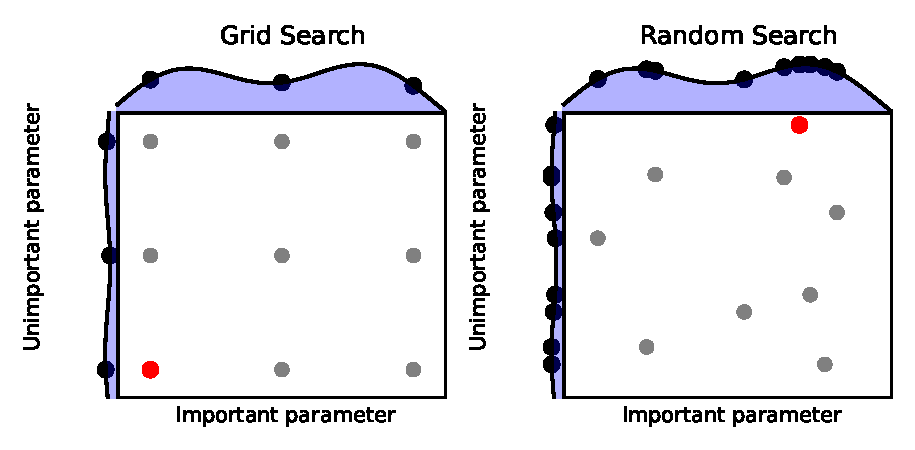
\includegraphics[scale=0.8]{img/grid_vs_rs.pdf}
    \caption{A visual comparison of Grid Search versus Random Search. Suppose that we optimize a function with two parameters and the function is the sum of the functions defined for each parameter. The best configuration found after nine trials is highlighted in red. If one of the parameters is not important, grid search wastes resources by repeatedly evaluating similar configurations. }
    \label{fig:grid}
\end{figure}

\paragraph{Quasi-random search} If our budget is low then quasi-random search might be the better option. It works by generating a low-discrepancy sequence. Intuitively, a low-discrepancy sequence covers the whole domain evenly. Therefore, the search space is better covered even with a small number of samples. In the Deep learning tuning playbook, the authors recommend using quasi-random search over grid search and random search for the initial exploration of the hyperparameter space.



\section{Bayesian optimization}
% Going from model-less to model-based approaches
So far, we have seen model-less approaches, where each trial is independent. This approach offers some advantages, like parallelization and simplicity of implementation, but it is quite inefficient. Information obtained from previous trials is not used in any way to guide the search. Bayesian optimization methods build and use an internal model of the learning algorithm's generalization performance. Bayesian optimization is widely covered in literature, we will use the work of Brochu et al.~\cite{brochu2010tutorial} and Frazier~\cite{frazier2018tutorial} for the definitions and the description of the method.

% What is BO and history
% Before mockus was Kushner 1964 and Zilinkas 1975 - 2nd page of Frazier 2018
In general, Bayesian optimization is a class of optimization methods focused on optimizing a real-valued objective function \[ \max_{x\in A} f(x). \] The method got its name from the Bayes' theorem, which is applied by stating that the posterior probability of a model M given observations E is proportional to the likelihood of E given M multiplied by the prior probability of M \[ P(M \given E) \propto P(E \given M)P(M).\] The foundations were laid for Bayesian Optimization by Jonas Mockus~\cite{mockus1974bayesian} in the 1970s and 1980s, but it was not until the early 2000s that Bayesian Optimization got applied to machine learning by Carl Edward Rasmussen~\cite{rasmussen2006gaussian}. Since then, it has become arguably the most prominent advanced technique for hyperparameter optimization, studied by countless groups and being implemented in many popular hyperparameter optimization frameworks.

% BO algorithm introduction
The basic loop of a Bayesian optimization algorithm is simple as shown in Algorithm \ref{alg:bo}. First, the internal model is used to suggest the next hyperparameter configuration to try. This query is much cheaper than evaluating the objective function. We can think of the suggestion as the most promising configuration given the previous observations. More precisely, the algorithm maximizes an \textit{acquisition function} $a$ defined from the \textit{surrogate model}. Then the objective function is evaluated at this configuration and the observed result is added to a database. The surrogate is updated using the database with the new observation and the process is repeated until some stopping condition is triggered, e.g.\ the algorithm runs out of budget.


\begin{algorithm}
    \caption{Bayesian Optimization}
    \begin{algorithmic}[1]
    % \State {\textbf{Initialize}:} Gaussian process prior $GP$, acquisition function $a$, data $\mathcal{D} = \{(x_i, y_i)\}_{i=1}^n$
    \For{$t = 1, \:  2, \ldots $}
        \State Find the next point $x_t$ to evaluate: $x_t = \argmax_{x} a(x \given \mathcal{D}_{1:t-1})$.
        \State Sample the objective function:  $y_t = f(x_t)+ \epsilon_t$.

        \State Augment the data: $\mathcal{D}_{1:t}= \{\mathcal{D}_{1:t-1}, \: (x_t, \: y_t)\}$.
        \State Update the surrogate model given the data $\mathcal{D}_{1:t}$.
    \EndFor
    %\State \textbf{Return} the best point found (e.g., with the lowest $y$)
    \end{algorithmic}
    %\caption{}
    \label{alg:bo}
\end{algorithm}

% Practical considerations - objective function
Before we dive deeper into Bayesian Optimization, let us deal with some practical considerations and properties of the objective function and the feasible set. Since we have defined the hyperparameter optimization problem as minimization of the loss function, we can assume that $f$ is defined as $f(\lambda)=-\mathcal{L}(\lambda)$. Maximizing this function is equivalent to minimizing the original function. We also assume that the objective function is continuous. When we evaluate $f$, we observe only $f(x)$ and no first- or second-order derivatives, which would allow us to use a wider array of optimization methods. We do not know nor assume that $f$ has any special structure like concavity or linearity. To summarize, we can say that Bayesian Optimization is designed for black-box derivative-free global optimization.

% Objective assumptions - Lipschitz-continuous.
% We assume that the objective is Lipschitz-continuous. That is, there exists some constant $C$ such that for all $x_1,x_2\in A: ||f(x_1)-f(x_2)|| \leq C||x_1-x_2||$. The constant $C$ may be unknown.

% Practical considerations - feasible set
We assume further that all inputs $x$ are real-valued, which is not the case for all hyperparameters, and we will address this issue later. Finally, we assume the feasible set $A$ to be a hyper-rectangle $\{ x \in \R \mid a_i \leq x_i \leq b_i \}$, which makes it easy to assess membership.

% Where was Bayesian optimization used?

% General BO Summary
The two main components of a Bayesian Optimization algorithm are a Bayesian statistical model and an acquisition function. The model approximates the objective function including the uncertainty over its predictions and the acquisition function is used for choosing configurations to evaluate. We will go through both of these components in greater detail. First, we will introduce the commonly used acquisition functions, and then we will show three different models.

\subsection{Acquisition functions}
The purpose of an acquisition function is to guide the search. It would be possible to find the predictive mean of the surrogate and sample a configuration that maximizes the mean, but the strength of Bayesian optimization is that it expresses uncertainty. Acquisition functions are designed to take advantage of uncertainty and balance exploration versus exploitation. The acquisition function value might be high if the objective function predicted value is high, but also if the uncertainty of the model is high; the area is not well explored yet but promising. We assume that we have a Bayesian statistical model that for any $x$ in the domain outputs a prediction $y \sim \mathcal{N}(\mu(x), \sigma^2(x))$.

\subsubsection{Upper Confidence Bound}

\begin{figure}
    \centering
    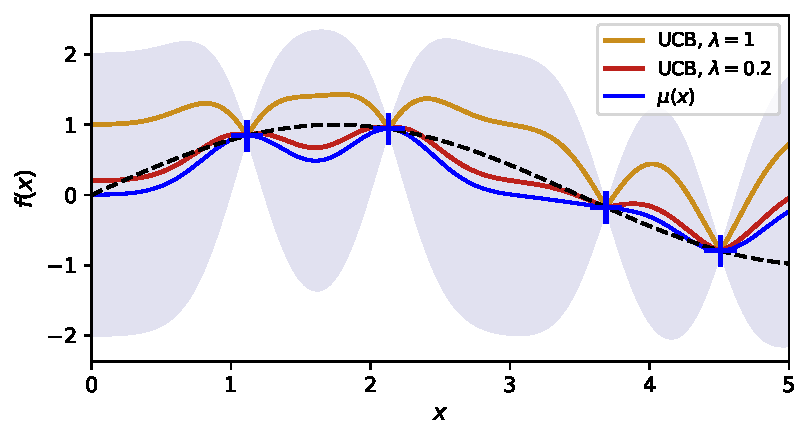
\includegraphics[scale=0.8]{img/ucb_example.pdf}
    \caption{An UCB acquisition function with two $\lambda$ settings demonstrated on a Bayesian model predicting mean $\mu(x)$, and variance (the light blue corresponds to two standard deviations from the mean), fitted to the black true function with four noisy observations.}
    \label{fig:ucb}
\end{figure}

Probably the simplest acquisition function is the Upper Confidence Bound (UCB). Given a mean $\mu(x)$ and a variance $\sigma(x)$, the UCB is calculated as
\[
    \text{UCB}(x) = \mu(x) + \lambda \sigma(x),
\]
where $\lambda$ is an exploration parameter. The smaller the $\lambda$, the more the UCB exploits regions that are known to yield good solutions and vice versa. The UCB acquisition function is illustrated in Figure~\ref{fig:ucb}.

\subsubsection{Probability of Improvement}
Let $y^*=\max_{i\in[1..n]} f(x_i)$ be the value of the best evaluated point so far after $n$ iterations and let $x$ be the next point we consider sampling. We define an improvement random variable as
\[
    I(x) \coloneq \max(f(x) - y^*),0).
\]

The probability of improvement acquisition function assigns to each candidate $x$ the probability of $I(x) > 0$. We can write
\[
    PI(x) = P(I(x) > 0) = P(f(x) > y^*) = 1-P(f(x) \leq y^*).
\]
Since we assume that $f(x)$ is normally distributed, then the PI is calculated from the cumulative density function $\Phi$ of normal distribution. We remind that for $X \sim \mathcal{N}(\mu,\sigma^2)$, we calculate $P(X \leq x)$ as $\Phi ((x-\mu)/\sigma )$. We also use the property $1-\Phi(x)=\Phi(-x)$. Therefore, the PI is calculated as follows:

\[
    PI(x) = 1 - \Phi\left(\frac{y^*-\mu(x)}{\sigma(x)}\right) = \Phi\left(\frac{\mu(x)-y^*}{\sigma(x)}\right).
\]

The problem with PI is that it does not factor in the magnitude of improvement. In the standard form, PI cares only about being as certain as possible about improving upon the incumbent solution. This often results in PI suggesting points close to the optimum, i.e.\ PI is biased towards exploitation. This problem is alleviated by adding a new parameter $\xi$, which forces PI to consider only points that are by at least $\xi$ better than the incumbent:
\[
    PI(x)=P(I(x)>\xi)
\]

\subsubsection{Expected improvement}
Expected improvement (EI)~\cite{jones1998efficient} enhances PI by considering the magnitude of improvement as well as the probability of improvement. That is achieved by taking the expected value of $I(x)$. Using the assumption that $I(x)$ is normally distributed, the density of $I(x)$ for a specific value of improvement, $I$, is given by
\[
\frac{1}{\sqrt{2 \pi}\sigma(x)} \text{exp}\left(-\frac{(\mu(x)-y^*-I)^2}{2\sigma^2(x)}\right).
\]
\xxx{Is the random variable notation used correctly here for $I(x)$? Is it a problem that we cut off the improvement at 0?}

The expected value is calculated by integrating the density function multiplied by the improvement:
\[ EI(x) = \mathbb{E}[I(x)] = \int_{I=0}^{I=\infty} I\frac{1}{\sqrt{2 \pi}\sigma(x)} exp\left(-\frac{(\mu(x)-y^*-I)^2}{2\sigma^2(x)}\right) dI. \]
The analytical solution to this integral can be found in the literature~\cite{jones1998efficient} and it is as follows:
\[ EI(x) = (\mu(x)-y^*)\Phi(Z)+\sigma(x)\phi(Z), \]
where
\[ Z=\frac{\mu(x)-y^*}{\sigma(x),} \]
and $\phi$ is the density of the normal distribution.

Even the expected improvement can be extended with parameter $\xi$ as in the PI acquisition function. The role of this parameter stays the same; it enables us to balance exploration and exploitation. The modified acquisition function is
\[
EI(x) = (\mu(x)-y^*-\xi)\Phi(Z)+\sigma(x)\phi(Z), \]
where
\[ Z=\frac{\mu(x)-y^*-\xi}{\sigma(x)}. \]
 Expected improvement is a popular acquisition function that balances the exploration-exploitation trade-off well; it prioritizes exploring regions with a high probability of significantly improving upon the current best solution. We compare all the mentioned acquisition functions in Figure~\ref{fig:ei}.

 \begin{figure}
    \centering
    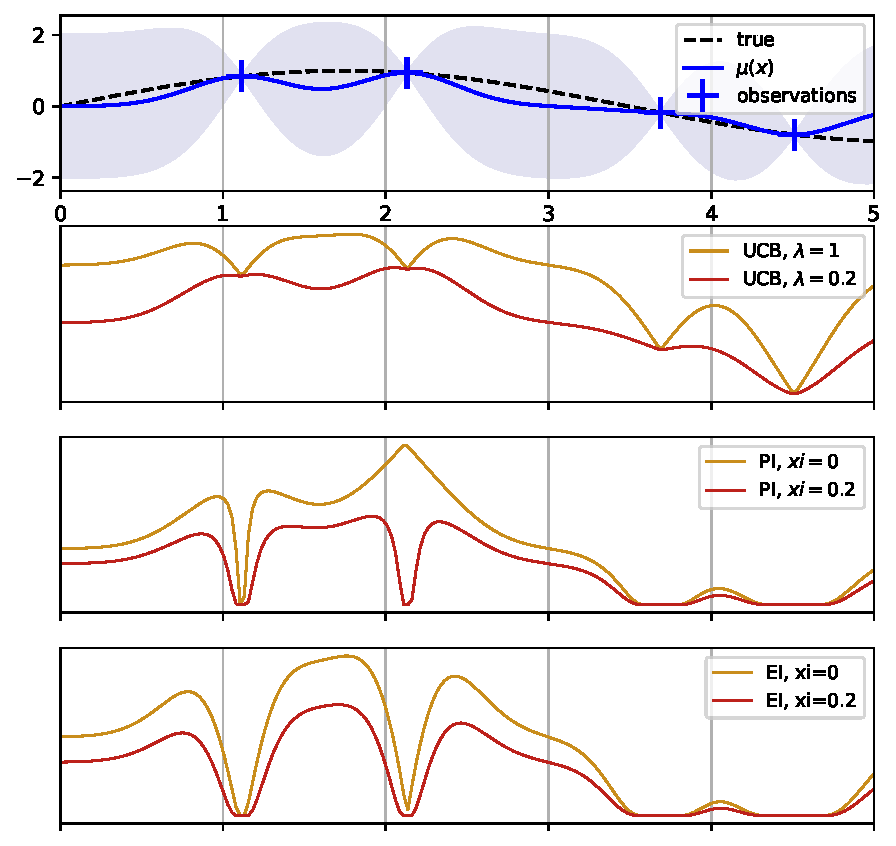
\includegraphics[scale=0.8]{img/acq_example.pdf}
    \caption{A comparison of different acquisition functions. The top image shows the real target function with a Bayesian model predicting mean and variance (the light blue area corresponds to two standard deviations). The other images show different acquisition functions from top to bottom: upper confidence bound, probability of improvement, and expected improvement.}
    \label{fig:ei}
\end{figure}

\xxx{Include other acquisitions if needed, like entropy search, or knowledge gradient}
% PI is for maximization
%Probability of improvement~\cite{kushner1964new} \[ \text{PI}(x) = P(y > y^* \given x) = \int_{y^*}^{\infty} p(y \given x) \, dy \]

%Entropy search
%Knowledge gradient

\newpage
\subsection{Gaussian Process Regression}
% Why is Gaussian process regression the default choice for Bayesian Optimization
The standard model in the Bayesian Optimization literature is the GP regression. An intuitive introduction to the topic was published by Jie Wang~\cite{wang2023intuitive}, and we use similar illustrations to present the topic. The definitions and the notation are taken from the textbook by Rasmussen~\cite{rasmussen2006gaussian}. There are many other machine learning algorithms for regression, but Gaussian processes offer a unique mix of properties that make them the natural choice. One of the most important properties of GPs is that they quantify the uncertainty, which allows us to incorporate it into our sampling strategy --- the areas with the most uncertainty should likely be explored more, or similar heuristic strategy. Another advantage is the possibility of incorporating our prior beliefs about the objective function with the kernel function. As a result, Gaussian processes are remarkably efficient when the amount of data is limited. On the other hand, GPs do not scale well with large datasets, because of their $\mathcal{O}(n^3)$ complexity. In practice, GPs limit us to the number of samples in the order of hundreds.

\subsubsection{Gaussian distribution}
% Univariate normal distribution
In order to describe the Gaussian process regression, we will start with the basics. A random variable X is Gaussian or normally distributed with mean $\mu$ and variance $\sigma^2$ if its probability density function is: \[ P_X(x) = \frac{1}{\sqrt{2\pi} \sigma} \exp\left(-\frac{(x-\mu)^2}{2 \sigma^2}\right). \] We denote that a random variable is normally distributed as $X \sim \mathcal{N}(\mu, \sigma^2)$. For illustration, we have sampled 500 points randomly from a univariate normal distribution into a vector $x_1 =[x_1^1,x_1^2, \ldots,x_1^{500}]$. In Figure~\ref{fig:1} we plot a histogram of the points and fit a Gaussian distribution over them. We also plot the points vertically along the Y-axis, which is the first step towards the Gaussian process regression.

\begin{figure}
    \centering
    \begin{subfigure}{0.49\textwidth}
        \centering
        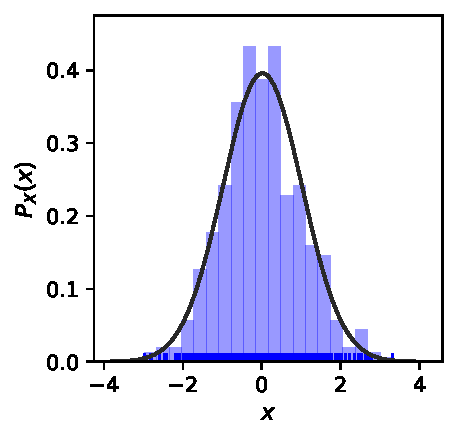
\includegraphics[scale=0.8]{img/1d_gaussian.pdf}
        \caption{Histogram of the samples with the fitted density as a black curve.}
%        \label{fig:f1}
    \end{subfigure}
    \hfill
    \begin{subfigure}{0.49\textwidth}
        \centering
        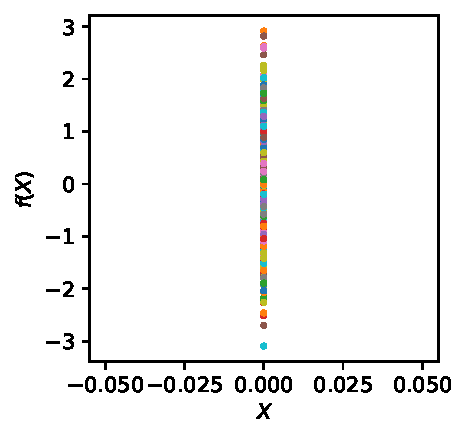
\includegraphics[scale=0.8]{img/1d_gaussian_projected.pdf}
        \caption{Random samples plotted vertically along the Y-axis with a fixed X coordinate.}
 %       \label{fig:f2}
    \end{subfigure}
    \caption{A visualization of sampling from a Gaussian distribution. A random variable $X \sim \mathcal{N}(0, 1)$ is sampled 500 times.}
    \label{fig:1}
\end{figure}

% Connecting several univariate Gaussian distributions
Similarly, we could sample several vectors $x_1,\ldots,x_n$ of points and plot them with a different x-coordinate as shown in Figure~\ref{fig:2}. If we connect the corresponding samples with a line, we could perform a regression task using these lines in the domain $[0,1]$. The issue is that the samples generating the lines are independent, making the predictions of no use. The key assumption for regression is that close points have similar values. Therefore, we have to find a way to introduce a correlation between the samples, preferably based on their distance.

% Connected distributions
\begin{figure}
    \centering
    \begin{subfigure}{0.49\textwidth}
        \centering
        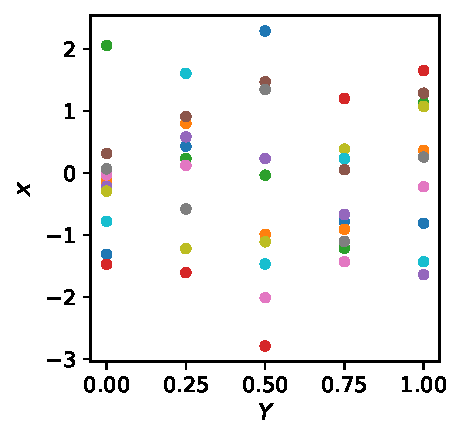
\includegraphics[scale=0.8]{img/10_gaussians.pdf}
        \caption{Random samples}
%        \label{fig:f1}
    \end{subfigure}
    \hfill
    \begin{subfigure}{0.49\textwidth}
        \centering
        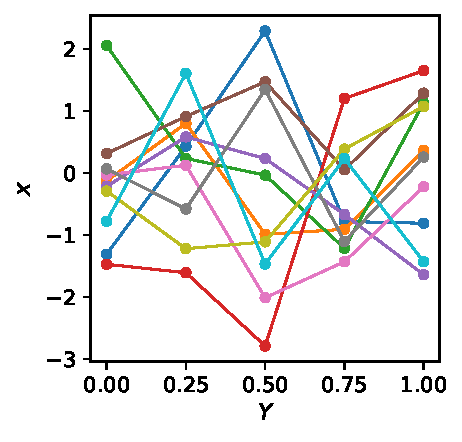
\includegraphics[scale=0.8]{img/10_gaussians_conn.pdf}
        \caption{Random samples connected by linear lines}
 %       \label{fig:f2}
    \end{subfigure}
    \caption{N=5 sampled random vectors, each with M=10 random samples drawn from a normal distribution. Samples from each vector are plotted along the Y-axis with the same X coordinate}
    \label{fig:2}
\end{figure}

% Multivariate normal distribution
A set of correlated, normally distributed random variables is described by the \textit{multivariate normal distribution} (MVN). We denote MVN as $\mathbf{X} \sim \mathcal{N}_k(\mathbf{\mu}, \mathbf{\Sigma})$, where $\mathbf{X}=(X_1,X_2,\ldots ,X_n)^T$ is a random vector, $\mathbf{\mu}= (\mu_1,\mu_2,\ldots , \mu_n)^T$ are the means and $\mathbf{\Sigma} \in  \R^{k \times k}$ is the covariance matrix. The $k$ is often omitted as the dimensions are usually clear from the context. The covariance matrix specifies the covariance between each pair of elements of a given random vector, with $\Sigma_{ij} = \text{cov}[X_i, X_j]$. The $\mathbf{\Sigma}$ is a symmetric and positive semi-definite matrix with variances on its main diagonal. Finally, the probability density function of k-dimensional MVN is defined as \[ \mathcal{N}(\mathbf{x} \given \mathbf{\mu}, \mathbf{\Sigma}) = \frac{1}{(2\pi)^{k/2} |\mathbf{\Sigma}|^{1/2}} \exp \left(-\frac{1}{2} (\mathbf{x} - \mathbf{\mu})^T \mathbf{\Sigma}^{-1} (\mathbf{x} - \mathbf{\mu}) \right). \]

% Bi-variate example

% Conditional MVN is also MVN
For regression, we are more interested in conditional probability rather than joint probability, as we want to make use of the observed data points. To get the conditional probability, we can partition the random vector $\mathbf{X}$ into $\mathbf{X_1}$ and $\mathbf{X_2}$. The conditional probability of $\mathbf{X_1}$ given $\mathbf{X_2}$ is also an MVN because a multivariate normal distribution is closed under conditioning. We will show the exact formulas in the description of Gaussian process regression.

%
\subsubsection{Kernels}
% Kernels in general - smoothens the functions
Using the multivariate normal distribution, we can correlate the points of our regression function. Instead of manually specifying the covariance matrix, we will use kernels. A kernel function measures the similarity between a pair of data points. This in turn impacts the smoothness of the regression functions --- we want close points to have similar function values, and we use the kernel function to determine the strength of the correlation.

% RBF kernel, Figure with samples with RBF covariance
A common choice is the squared exponential kernel, also called the Radial Basis Function (RBF) kernel, defined as \[ K(x, x') = exp \left( -  \frac{||x - x'||^2} {2 \sigma^2}\right). \] The kernel has a parameter $\sigma$ called the length scale. It controls how quickly the correlation between two points decays. The functions predicted by the kernel are smooth and infinitely differentiable. We have plotted samples of the twenty-variate normal distribution with RBF kernel as covariance function in Figure~\ref{fig:f3}. Note that the samples illustrated in Figure~\ref{fig:2} can also be viewed as being drawn from MVN distribution, but with an identity covariance function, which highlights the role of a kernel.

% Lines drawn using samples from Multivariate normal distribution
\begin{figure}
    \centering
    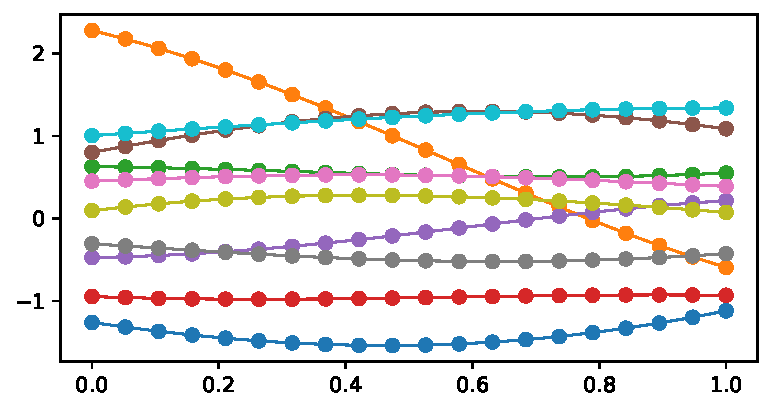
\includegraphics[scale=0.8]{img/20_gaussians_with_prior.pdf}
    \caption{Samples from the 20-VN distribution with RBF covariance.}
    \label{fig:f3}
\end{figure}
% For two separate figures, I would use minipage

% The 'kernel trick'

% Infinite dim MVN
We have now covered all the background necessary to get to Gaussian processes. We understand how the MVN is used with kernels to produce correlated predictions that look smoother when connected with lines. As we increase the dimensions of the MVN, the points will get closer and closer together in the domain of interest. For a truly smooth prediction spanning the whole domain, we use MVN distribution with infinite dimensions. % We call such functions \textit{kernelized prior functions}.


\subsubsection{Gaussian processes}
% Parametric vs non-parametric models
%Gaussian processes are a non-parametric model, meaning that there are no parameters that define the regression function such as $\theta_1$ and $\theta_2$ in a linear regression model $y = \theta_1 + \theta_2 x$. After a parametric model is trained, the predictions no longer depend on the training data and all the information is encapsulated in the parameters. Instead, non-parametric models do not assume any specific form for the relationship between independent and dependent variables and the model structure is determined by the data itself.

\begin{figure}
    \centering
    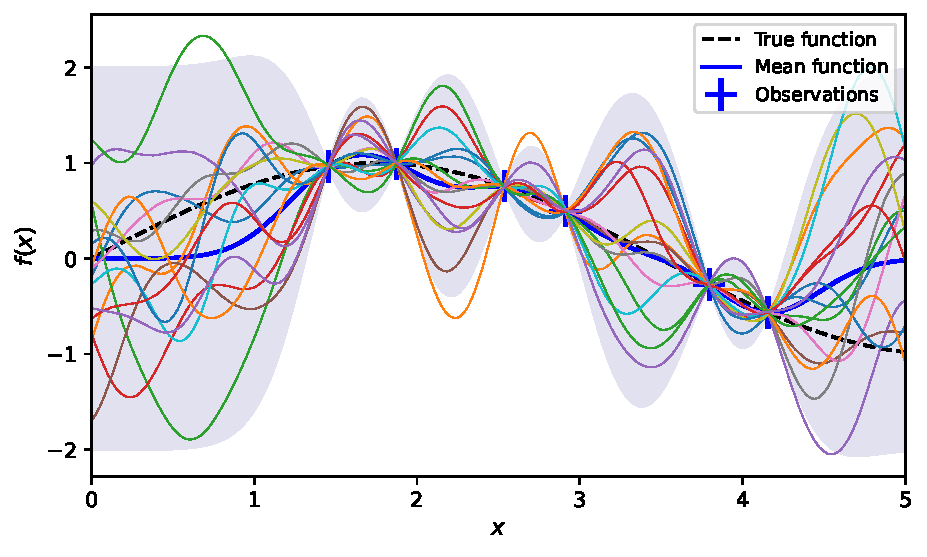
\includegraphics[scale=0.8]{img/gaussian_process.pdf}
    \caption{An example of Gaussian process regression. The black dashed line is the true target function. We drew six random samples and the function was evaluated at these points with noise (blue crosses). Then we sampled 15 functions from the posterior distribution given the test points. The blue line is the mean function and the light blue area is bounded at two standard deviations from the mean.}
    \label{fig:f4}
\end{figure}

% Introduction (infinite MVN), example
Gaussian processes are a generalization of MVN into infinite dimensions. The kernel specifies permissible functions which make up the prior distribution. The Gaussian process model defines a probability distribution over prior functions that fit the observed data. The concept is best illustrated in an example. In Figure~\ref{fig:f4}, we want to perform a regression task over the true (black) function. We are given six noisy observations. We can derive the (blue) mean function by calculating the posterior distribution and averaging over all functions weighted by their posterior probability. For the illustration of the posterior distribution, we can observe the light blue area marking two standard deviations from the mean. Lastly, the colorful functions are randomly sampled from the posterior distribution.

Let us define the Gaussian process formally. Let $\mathbf{X}=[\mathbf{x_1}, \ldots ,\mathbf{x_n}]$ represent the observed data points, $\mathbf{f}=[f(\mathbf{x_1}), \ldots ,f(\mathbf{x_n})]$ the function values, $\mathbf{\mu}=[m(\mathbf{x_1}),\ldots , m(\mathbf{x_n})]$ the mean function, and $K_{ij}=k(\mathbf{x_i}, \mathbf{x_j})$ the positive definite kernel function. The mean function represents a prior mean --- our initial belief about the average behavior of the function across the input space --- and is often just assumed to be $0$. Let us consider a regression task. We want to predict function values $\mathbf{f}(\mathbf{X}_*)$ at new points $\mathbf{X}_*$ using the Gaussian process regression. The joint distribution of $\mathbf{f}$ and $\mathbf{f_*}$ is given by
\[
\begin{bmatrix}
    \mathbf{f} \\ \mathbf{f}_*
    \end{bmatrix}
    \sim
    \mathcal{N} \left(
    \begin{bmatrix}
    m(\mathbf{X}) \\ m(\mathbf{X}_*)
    \end{bmatrix} ,
    \begin{bmatrix}
    \mathbf{K} & \mathbf{K}_* \\
    \mathbf{K}_*^T & \mathbf{K}_{**}
    \end{bmatrix}
    \right) \ ,
\]
where $\mathbf{K}=K(\mathbf{X},\mathbf{X})$, $\mathbf{K}_*=K(\mathbf{X},\mathbf{X}_*)$, $\mathbf{K}_{**}=K(\mathbf{X}_*,\mathbf{X}_*)$, and we assume that $(m(\mathbf{X}),m(\mathbf{X_*}))=\mathbf{0}$.

Since we solve the regression task, we are interested in the conditional distribution $P(\mathbf{f}_* \given \mathbf{f},\mathbf{X}, \mathbf{X_*})$, not the joint distribution. Using the formula for MVN conditional distribution, it can be derived from the joint distribution $P(\mathbf{f}_*,\mathbf{f} \given \mathbf{X}, \mathbf{X_*})$ as
\[ \mathbf{f}_*  \given  \mathbf{f}, \mathbf{X}, \mathbf{X_*} \sim \mathcal{N} \left(
    \mathbf{K}^T_* \mathbf{K}^{-1} \mathbf{f}, \ \mathbf{K}_{**} - \mathbf{K}^T_* \mathbf{K}^{-1} \mathbf{K}_*
 \right) \ .
 \]

 We often encounter noisy observations in practice, which is often the case for the hyperparameter optimization problem as well. We deal with noisy observations by assuming additive independent and identically distributed Gaussian noise $\epsilon$ with variance $\sigma_n^2$. The noise is incorporated into the prior as $\text{cov}(y)= \mathbf{K}+\sigma_n^2 \mathbf{I}$. Then the observations can be expressed as $y=f(\mathbf{x})+ \epsilon$. The joint distribution with noise is
 \[
\begin{bmatrix}
    \mathbf{y} \\ \mathbf{f}_*
    \end{bmatrix}
    \sim
    \mathcal{N} \left(
    \mathbf{0},
    \begin{bmatrix}
    \mathbf{K} + \sigma^2_n \mathbf{I} & \mathbf{K}_* \\
    \mathbf{K}_*^T & \mathbf{K}_{**}
    \end{bmatrix}
    \right) \ .
\]

Finally, the conditional distribution with noise is derived as
\[ \mathbf{\bar{f}}_* \given \mathbf{y}, \mathbf{X}, \mathbf{X_*} \sim \mathcal{N} \left(
    \mathbf{\bar{f}_*}, \text{cov}(\mathbf{f_*})
 \right) \ ,\]
 where

  \begin{align*}
  \mathbf{\bar{f}}_* &\overset{\Delta}{=} \mathbb{E}[ \mathbf{\bar{f}}_*  \given  \mathbf{y}, \mathbf{X}, \mathbf{X}_*] \\
                    &= \mathbf{K}^T_*[\mathbf{Κ} + \sigma^2_n \mathbf{I}]^{-1} \mathbf{y}\ \text{,} \\
          \text{cov}(\mathbf{f}_*)  &= \mathbf{K}_{**} - \mathbf{K}_*^T[\mathbf{K}+\sigma^2_n\mathbf{I}]^{-1}\mathbf{K}_* \ \text{.}
  \end{align*}

% Include the algorithm 2.1. from Rasmussen?


% General recommendations when to use GPR
Gaussian processes are best suited for optimization over continuous domains of less than 20 dimensions and when the number of function evaluations is very low. GPs tolerate stochastic noise in function evaluations~\cite{frazier2018tutorial}.

% "For continuous functions, Bayesian optimization typically works by assuming the unknown function was sampled from a Gaussian process and maintains a posterior distribution for this function as observations are made or, in our case, as the results of running learning algorithm experiments with different hyperparameters are observed (Practical Bayesian optimization 2012)"


% Good overview of Gaussian processes: \cite{brochu2010tutorial}.

% Practical BO of ML algorithms. They show how different kernels affect performance and describe algorithms that take into account the variable cost (duration) of learning algorithm experiments~\cite{snoek2012practical}.


\subsection{Tree-Structured Parzen Estimator}

Another popular Bayesian optimization method for hyperparameter optimization is the Tree-structured Parzen Estimator (TPE) introduced by Bergstra et al.~\cite{bergstra2011algorithms} As the name suggests, it is an extension of a Parzen estimator to a tree-structured search space. Therefore, a TPE can handle conditional parameters as well. A Parzen estimator, also known as a kernel density estimator (KDE), is a non-parametric method used to estimate the probability density function of a random variable based on a set of observed data points. Instead of assuming the underlying distribution and fitting it to the data, a Parzen estimator uses a kernel function to determine the shape and influence of each data point on the estimated probability density function.

In a TPE algorithm, two kernel density estimators are used. Keeping the notation from the original paper~\cite{bergstra2011algorithms}, we want to minimize the objective function $f(x)$ and the observations $\mathcal{D}$ are split into the better (lower) group $\mathcal{D}^{(l)}$ and the worse (greater) group $\mathcal{D}^{(g)}$ based on their objective value; for illustration see the top left part of Figure~\ref{fig:tpe}. More precisely, the top-quantile $\gamma$ is computed in each iteration based on the number of observations $N=|\mathcal{D}|$ and $y^{\gamma}$ is the top-$\gamma$-quantile objective value in the set of observations $\mathcal{D}$. Observations with $y\leq y^\gamma$ are assigned into the $\mathcal{D}^{(l)}$, and observations with $y > y^\gamma$ to the $\mathcal{D}^{(g)}$. The subsets are used to model $p(\mathbf{x} \given y, \mathcal{D})$ with the assumption:
\begin{equation} (\mathbf{x} \given y, \mathcal{D})\coloneq  \left\{
  \begin{array}{ll}
        p(\mathbf{x} \given \mathcal{D}^{(l)}) \quad  &(y \leq y^\gamma) \\
        p(\mathbf{x} \given \mathcal{D}^{(g)}) \quad  &(y > y^\gamma)
  \end{array}
  \right. .
  \label{eqn:tpe:assumption}
\end{equation}

\begin{figure}
    \centering
    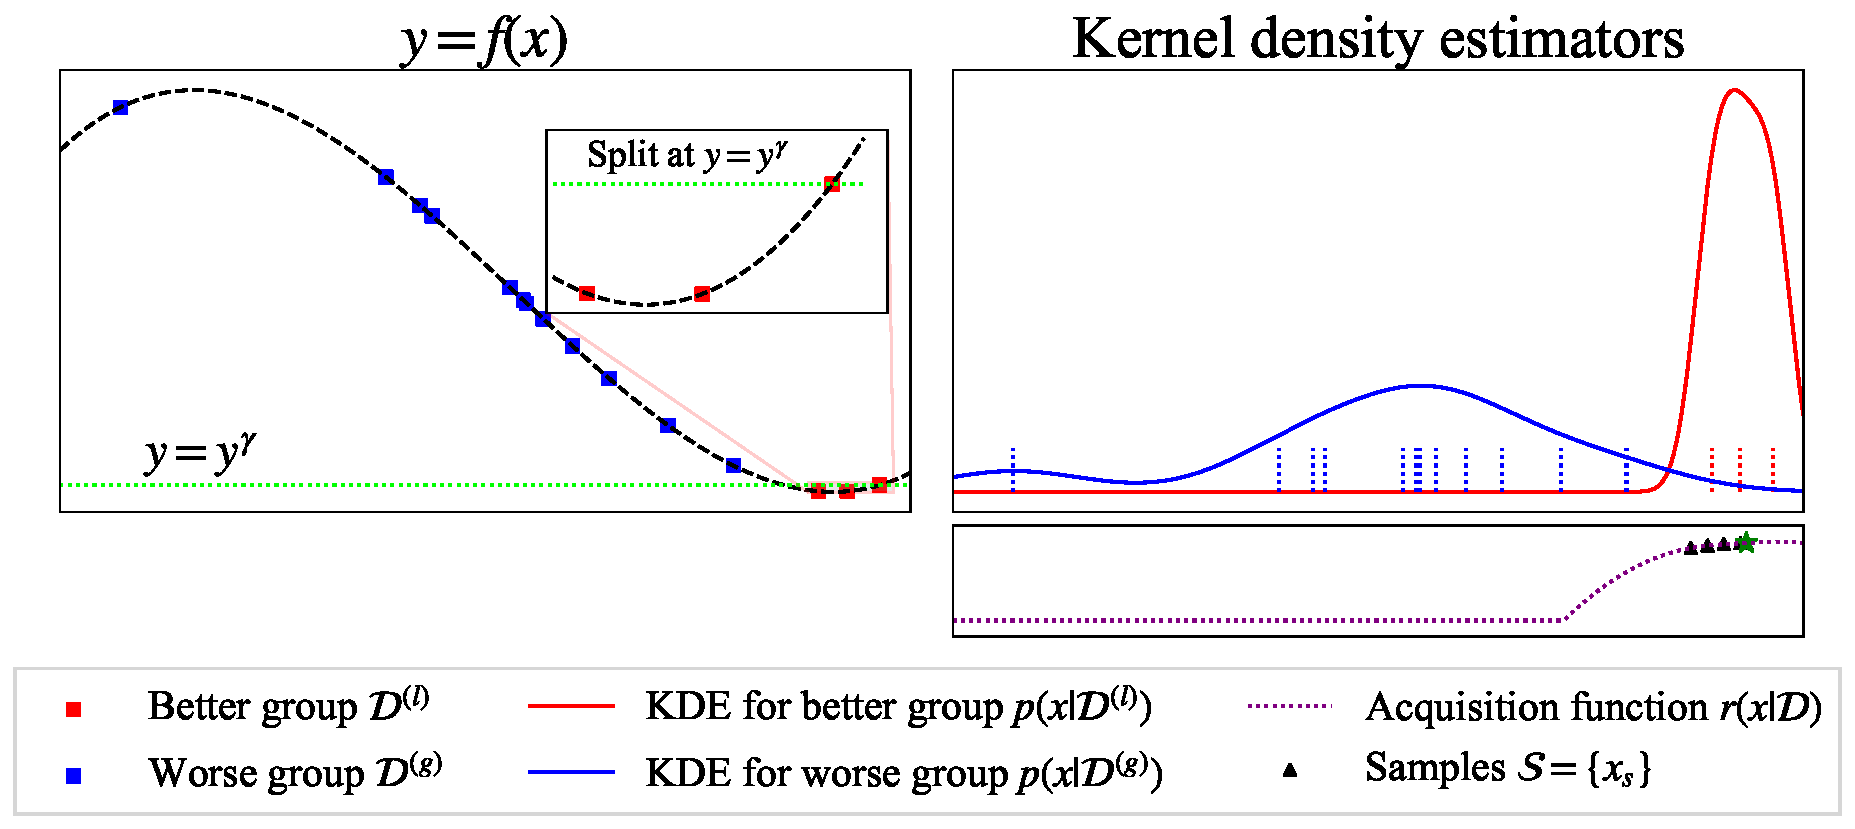
\includegraphics[scale=0.40]{img/tpe-conceptual.pdf}
    \caption{Example of the TPE algorithm. We are searching for the minimum of the target (black) function. The observations are split into $D^{(l)}$ and $D^{(g)}$ by the green line on the objective value of observations. For each group, a kernel density estimation is calculated. The acquisition function is derived from the densities and the algorithm chooses the next point to sample by finding the maximum (Source: Figure 1 from Watanabe~\cite{watanabe2023tree}).}
    \label{fig:tpe}
\end{figure}

Now we can show how the kernel density estimations from the equation above are calculated. Let us assume the $D$ is sorted by $y_n$ such that $y_1 \leq y_2 \leq \cdots \leq y_N$. Then the KDEs are estimated as


\begin{equation}
    \begin{split}
   p(\mathbf{x} \given \mathcal{D}^{(l)}) &= w_0^{(l)} p_0(\mathbf{x}) + \sum_{n=1}^{N^{(l)}}w_n k(\mathbf{x},\mathbf{x}_n \given b^{(l)}), \\
   p(\mathbf{x} \given \mathcal{D}^{(g)}) &= w_0^{(g)} p_0(\mathbf{x}) + \sum_{n=N^{(l)}+1}^{N}w_n k(\mathbf{x},\mathbf{x}_n \given b^{(g)}),
    \end{split}
    \label{eqn:tpe:kdes}
\end{equation}

where $k$ is a kernel function, the weights $\{ w_n \}_{n=1}^N$ are recomputed every iteration, $b^{(l)},b^{(g)} \in \R_+$ are the bandwidth and $p_0$ is non-informative prior. The KDEs are illustrated in the top right part of Figure~\ref{fig:tpe}.

The last part of the algorithm yet to be described is the acquisition function. It is calculated from the KDEs using the assumption from Eq.~\ref{eqn:tpe:assumption} as
\[
\mathbb{P}(y \leq y^\gamma \given \mathbf{x},\mathcal{D}) \overset{\text{rank}}{\simeq} r(\mathbf{x} \given \mathcal{D}) \coloneq  \frac{p(\mathbf{x} \given \mathcal{D}^{(l)})}{p(\mathbf{x} \given \mathcal{D}^{(g)})} ,
\]
where the $\overset{\text{rank}}{\simeq}$ symbol means the order isomorphic between the left-hand side and the right-hand side. See Figure~\ref{fig:tpe} for illustration. The detailed pseudocode is provided in Algorithm~\ref{tpe-algo}.
% TODO: Edit out missing references in the pseudocode.

\subfile{./alg/tpe-algo.tex}

\subsubsection{Components and control parameters}
\xxx{In this section, we will look at how the different components and control parameters change the behavior of the algorithm}. We start with the \emph{splitting algorithm}, which is used to split the observations $\D$ into $\Dl$ and $\Dg$. Weighting Algorithm. Kernel Functions (numerical, categorical, univariate vs multivariate). Bandwidth. Non-informative prior. \xxx{Will I have to go into such a details?}

\subsection{Random Forest}
The last Bayesian optimization surrogate that we are going to introduce is the random forest model. This approach was first introduced by Hutter et al.~\cite{hutter2010sequential} as SMAC, which stands for Sequential Model-based Algorithm Configuration. It was published as an alternative to the Gaussian processes for the general algorithm configuration problem, approximately at the same time as the TPE.\@ The random forest surrogate is still widely used, mostly in the updated SMAC3 Python package~\cite{smac3}.

Random forest~\cite{breiman2001random} is a machine learning method for classification and regression that trains an ensemble of decision trees and predicts the combined value from all the decision trees during inference. In SMAC, random forests are used for regression to directly model the objective function. The advantage of using regression trees is that they perform well on categorical input data, where Gaussian processes usually struggle \xxx{(add citation)}. The model is trained by randomly sampling $n$ data points with repetition for each of $B$ regression trees. At each split point in a tree, only a random subset of features is considered. The default is $5/6$ of all features. The default number of regression trees in the algorithm $B$ is set to $10$. There is one more parameter $n_{min}$ for the minimal number of data points required to split a node. This parameter is set to $n_{min}=10$ by default.

Prediction for a new data point is the empirical mean of individual trees' predictions. A prediction of a single tree is usually the mean of the data points in the leaf that corresponds to the input configuration, but the authors implement an option for a user-defined prediction function as well. The algorithm also calculates the empirical variance from the predictions of the individual trees. To select the next configuration to evaluate, the expected improvement acquisition function is maximized. SMAC solves the maximization problem by a multi-start local search. According to the authors, this method provides better results than random sampling.
% Could write a little more about the local search.
